\documentclass[border=90pt]{standalone}

\usepackage{tikz}
\usetikzlibrary{hobby,spath3}

\def\firstcharacter#1{\expandafter\firstcharacterA#1{}\end}
\def\firstcharacterA#1#2\end{#1}
\usetikzlibrary{colorbrewer}


\usetikzlibrary{calc}
\usetikzlibrary{patterns}

\usetikzlibrary{patterns.meta}

\pgfdeclarepattern{
    name=hatch,
    parameters={\hatchsize,\hatchangle,\hatchlinewidth},
    bottom left={\pgfpoint{-.1pt}{-.1pt}},
    top right={\pgfpoint{\hatchsize+.1pt}{\hatchsize+.1pt}},
    tile size={\pgfpoint{\hatchsize}{\hatchsize}},
    tile transformation={\pgftransformrotate{\hatchangle}},
    code={
        \pgfsetlinewidth{\hatchlinewidth}
        \pgfpathmoveto{\pgfpoint{-.1pt}{-.1pt}}
        \pgfpathlineto{\pgfpoint{\hatchsize+.1pt}{\hatchsize+.1pt}}
        \pgfpathmoveto{\pgfpoint{-.1pt}{\hatchsize+.1pt}}
        \pgfpathlineto{\pgfpoint{\hatchsize+.1pt}{-.1pt}}
        \pgfusepath{stroke}
    }
}

\tikzset{
    hatch size/.store in=\hatchsize,
    hatch angle/.store in=\hatchangle,
    hatch line width/.store in=\hatchlinewidth,
    hatch size=5pt,           % Smaller hatch size for fewer lines
    hatch angle=45pt,         % More angle to spread lines
    hatch line width=.5pt,    % Thin lines
}



\begin{document}
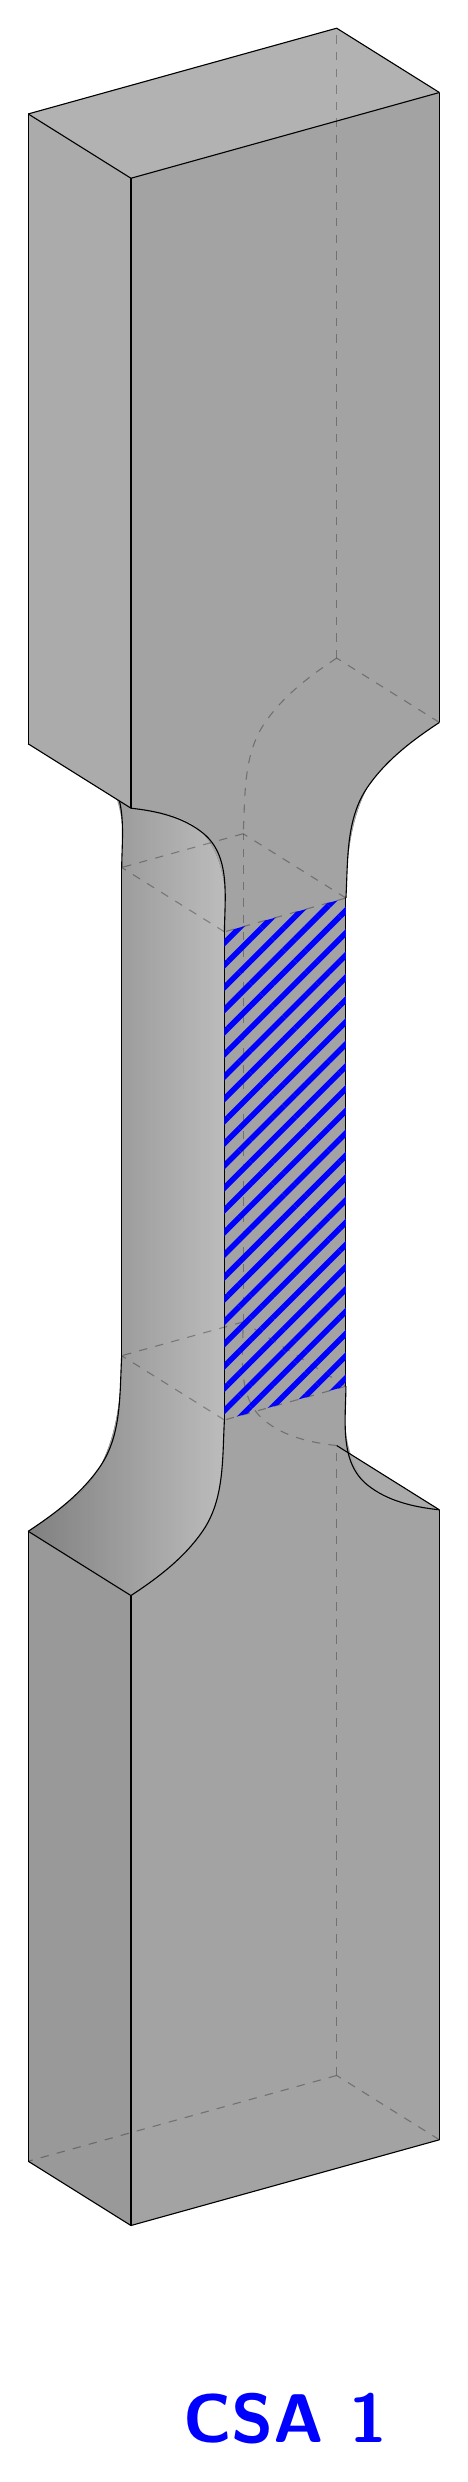
\begin{tikzpicture}[rotate around y=225, use Hobby shortcut]
    \large
    \def\width{4}
    \def\gap{10}
    \def\main{8}
    \def\curvy{1.9}
    \def\depth{3}
    
    \def\n{3.3}
    \def\z{1/\n}
    \pgfmathsetmacro{\s}{1-\z}
    
    \coordinate (A) at (0,\main,0);
    \coordinate (B) at (\width*\z-\width*\z*0.23,\main+\curvy-\curvy*0.7,0);
    \coordinate (C) at (\width*\z,\main+\curvy,0);
    
    \coordinate (A2) at (\width,\main,0);
    \coordinate (B2) at (\width*\s+\width*\z*0.23,\main+\curvy-\curvy*0.7,0);
    \coordinate (C2) at (\width*\s,\main+\curvy,0);
    
    \coordinate (A3) at (0,\main+\gap,0);
    \coordinate (B3) at (\width*\z-\width*\z*0.23,\main+\gap-\curvy+\curvy*0.7,0);
    \coordinate (C3) at (\width*\z,\main+\gap-\curvy,0);
    
    \coordinate (A4) at (\width,\main+\gap,0);
    \coordinate (B4) at (\width*\s+\width*\z*0.23,\main+\gap-\curvy+\curvy*0.7,0);
    \coordinate (C4) at (\width*\s,\main+\gap-\curvy,0);
    
    % Back variation with \depth (subtracting \depth from the z-coordinate)
    \coordinate (A') at (0,\main,\depth);
    \coordinate (B') at (\width*\z-\width*\z*0.23,\main+\curvy-\curvy*0.7,\depth);
    \coordinate (C') at (\width*\z,\main+\curvy,\depth);
    
    \coordinate (A2') at (\width,\main,\depth);
    \coordinate (B2') at (\width*\s+\width*\z*0.23,\main+\curvy-\curvy*0.7,\depth);
    \coordinate (C2') at (\width*\s,\main+\curvy,\depth);
    
    \coordinate (A3') at (0,\main+\gap,\depth);
    \coordinate (B3') at (\width*\z-\width*\z*0.23,\main+\gap-\curvy+\curvy*0.7,\depth);
    \coordinate (C3') at (\width*\z,\main+\gap-\curvy,\depth);
    
    \coordinate (A4') at (\width,\main+\gap,\depth);
    \coordinate (B4') at (\width*\s+\width*\z*0.23,\main+\gap-\curvy+\curvy*0.7,\depth);
    \coordinate (C4') at (\width*\s,\main+\gap-\curvy,\depth);
    
    
    % Back face fill
    \fill[black!40] 
    (0,0,\depth) -- (\width,0,\depth) -- (\width,\main,\depth) 
    to[hobby,tension=3] (\width,\main,\depth) .. (\width*\s+\width*\z*0.23,\main+\curvy-\curvy*0.7,\depth) .. (\width*\s,\main+\curvy,\depth) -- 
    (\width*\s,\main+\gap-\curvy,\depth) 
    to[hobby,tension=3] (\width*\s,\main+\gap-\curvy,\depth)  .. (\width*\s+\width*\z*0.23,\main+\gap-\curvy+\curvy*0.7,\depth) .. (\width,\main+\gap,\depth) --
    (\width,2*\main+\gap,\depth) -- (0,2*\main+\gap,\depth) -- 
    (0,\main+\gap,\depth) to[hobby,tension=3] (0,\main+\gap,\depth) .. (\width*\z-\width*\z*0.23,\main+\gap-\curvy+\curvy*0.7,\depth) .. (\width*\z,\main+\gap-\curvy,\depth) --
    (\width*\z,\main+\curvy,\depth) to[hobby,tension=3] (\width*\z,\main+\curvy,\depth) .. (\width*\z-\width*\z*0.23,\main+\curvy-\curvy*0.7,\depth) .. (0,\main,\depth) --
    cycle;
    
    % Curves fills with refined fades
    \fill[left color=gray!80, middle color=gray!50, right color=gray!20, opacity=0.8] 
    (A) to[hobby,tension=3] (A) .. (B) .. (C) -- (C3) to[hobby,tension=3] (C3) .. (B3) .. (A3) -- 
    (A3') to[hobby,tension=3] (A3') .. (B3') .. (C3') --
    (C') to[hobby,tension=3] (C') .. (B') .. (A') -- cycle;
    
    \fill[left color=gray!80, middle color=gray!50, right color=gray!20, opacity=0.8] 
    (A2) to[hobby,tension=3] (A2) .. (B2) .. (C2) -- (C4) to[hobby,tension=3] (C4) .. (B4) .. (A4) -- 
    (A4') to[hobby,tension=3] (A4') .. (B4') .. (C4') --
    (C2') to[hobby,tension=3] (C2') .. (B2') .. (A2') -- cycle;
    
    
    \draw[-,hobby,tension=3] (A2') .. (B2') .. (C2');
    \draw[-,hobby,tension=3] (A4') .. (B4') .. (C4');
    
    % Fill for bottom rectangle section
    \fill[black!33] 
    (0,0,0) -- (\width,0,0) -- (\width,0,\depth) -- (0,0,\depth) -- cycle;
    \fill[black!33] 
    (0,0,0) -- (0,\main,0) -- (0,\main,\depth) -- (0,0,\depth) -- cycle;
    \fill[black!40] 
    (\width,0,0) -- (\width,\main,0) -- (\width,\main,\depth) -- (\width,0,\depth) -- cycle;
    
    % Fill for top rectangle section
    \fill[black!30] 
    (0,2*\main+\gap,0) -- (\width,2*\main+\gap,0) -- (\width,2*\main+\gap,\depth) -- (0,2*\main+\gap,\depth) -- cycle;
    \fill[black!30] 
    (0,\main+\gap,0) -- (0,2*\main+\gap,0) -- (0,2*\main+\gap,\depth) -- (0,\main+\gap,\depth) -- cycle;
    \fill[black!33] 
    (\width,\main+\gap,0) -- (\width,2*\main+\gap,0) -- (\width,2*\main+\gap,\depth) -- (\width,\main+\gap,\depth) -- cycle;
    
    
    
    % Front face fill
    \fill[black!36] 
    (0,0,0) -- (\width,0,0) -- (\width,\main,0) 
    to[hobby,tension=3] (A2) .. (B2) .. (C2) -- 
    (\width*\s,\main+\gap-\curvy,0) 
    to[hobby,tension=3] (C4) .. (B4) .. (A4) --
    (\width,2*\main+\gap,0) -- (0,2*\main+\gap,0) -- 
    (0,\main+\gap,0) to[hobby,tension=3] (A3) .. (B3) .. (C3) --
    (\width*\z,\main+\curvy,0) to[hobby,tension=3] (C) .. (B) .. (A) --
    cycle;
    \draw[hobby,tension=3] (A) .. (B) .. (C);
    \draw[hobby,tension=3] (A2) .. (B2) .. (C2);
    \draw[hobby,tension=3] (A3) .. (B3) .. (C3);
    \draw[hobby,tension=3] (A4) .. (B4) .. (C4);
    \draw[dashed, opacity=0.3,hobby,tension=3] (A3') .. (B3') .. (C3');
    \draw[dashed, opacity=0.3,hobby,tension=3] (A') .. (B') .. (C');
    % Front face outline
    
    \draw[-] (0,0,0) -- (\width,0,0);
    \draw[-] (0,0,0) -- (0,\main,0);
    \draw[-] (\width*\z,\main+\curvy,0) -- (\width*\z,\main+\gap-\curvy,0);
    \draw[-] (0,\main+\gap,0) -- (0,2*\main+\gap,0);
    \draw[-] (0,2*\main+\gap,0) -- (\width,2*\main+\gap,0);
    \draw[-] (\width,2*\main+\gap,0) -- (\width,\main+\gap,0);
    \draw[-] (\width*\s,\main+\curvy,0) -- (\width*\s,\main+\gap-\curvy,0);    
    \draw[-] (\width,0,0) -- (\width,\main,0);
    
    
    
    
    
    % Back face outline
    
    
    \draw[dashed, opacity=0.3] (\width*\z,\main+\curvy,\depth) -- (\width*\z,\main+\gap-\curvy,\depth);
    \draw[-] (\width*\s,\main+\curvy,\depth) -- (\width*\s,\main+\gap-\curvy,\depth);
    \draw[dashed, opacity=0.3] (0,0,\depth) -- (\width,0,\depth);
    \draw[dashed, opacity=0.3] (0,0,\depth) -- (0,\main,\depth);
    \draw[-] (\width,0,\depth) -- (\width,\main,\depth);
    \draw[dashed, opacity=0.3] (0,\main+\gap,\depth) -- (0,2*\main+\gap,\depth);
    \draw[-] (0,2*\main+\gap,\depth) -- (\width,2*\main+\gap,\depth);
    \draw[-] (\width,2*\main+\gap,\depth) -- (\width,\main+\gap,\depth);
    
    
    
    % Connect front and back faces
    %botom
    \draw[-] (\width,\main,0) -- (\width,\main,\depth);
    \draw[-] (\width,0,0) -- (\width,0,\depth);
    \draw[dashed, opacity=0.3] (0,0,0) -- (0,0,\depth);
    \draw[-] (0,\main,0) -- (0,\main,\depth);
    %top
    \draw[-] (\width,\main+\gap,0) -- (\width,\main+\gap,\depth);
    \draw[-] (\width,2*\main+\gap,0) -- (\width,2*\main+\gap,\depth);
    \draw[-] (0,2*\main+\gap,0) -- (0,2*\main+\gap,\depth);
    \draw[dashed, opacity=0.3] (0,\main+\gap,0) -- (0,\main+\gap,\depth);
    
    
    
    %curves
    \draw[dashed, opacity=0.3] (C) -- (C2);
    \draw[dashed, opacity=0.3] (C3) -- (C4);
    \draw[dashed, opacity=0.3] (C') -- (C2');
    \draw[dashed, opacity=0.3] (C3') -- (C4');
    \draw[dashed, opacity=0.3] (C) -- (C');
    \draw[dashed, opacity=0.3] (C2) -- (C2');
    \draw[dashed, opacity=0.3] (C3) -- (C3');
    \draw[dashed, opacity=0.3] (C4) -- (C4');
    
    
    \fill[pattern={Lines[
        distance=2mm,
        angle=45,
        line width=0.7mm
        ]},
    pattern color=blue
    ] (C2) -- (C) -- (C3) -- (C4) -- cycle;
   \node at (2,-3,0) {\Huge \color{blue}\textbf{\textsf{CSA 1}}};
\end{tikzpicture}
\vspace{5em}
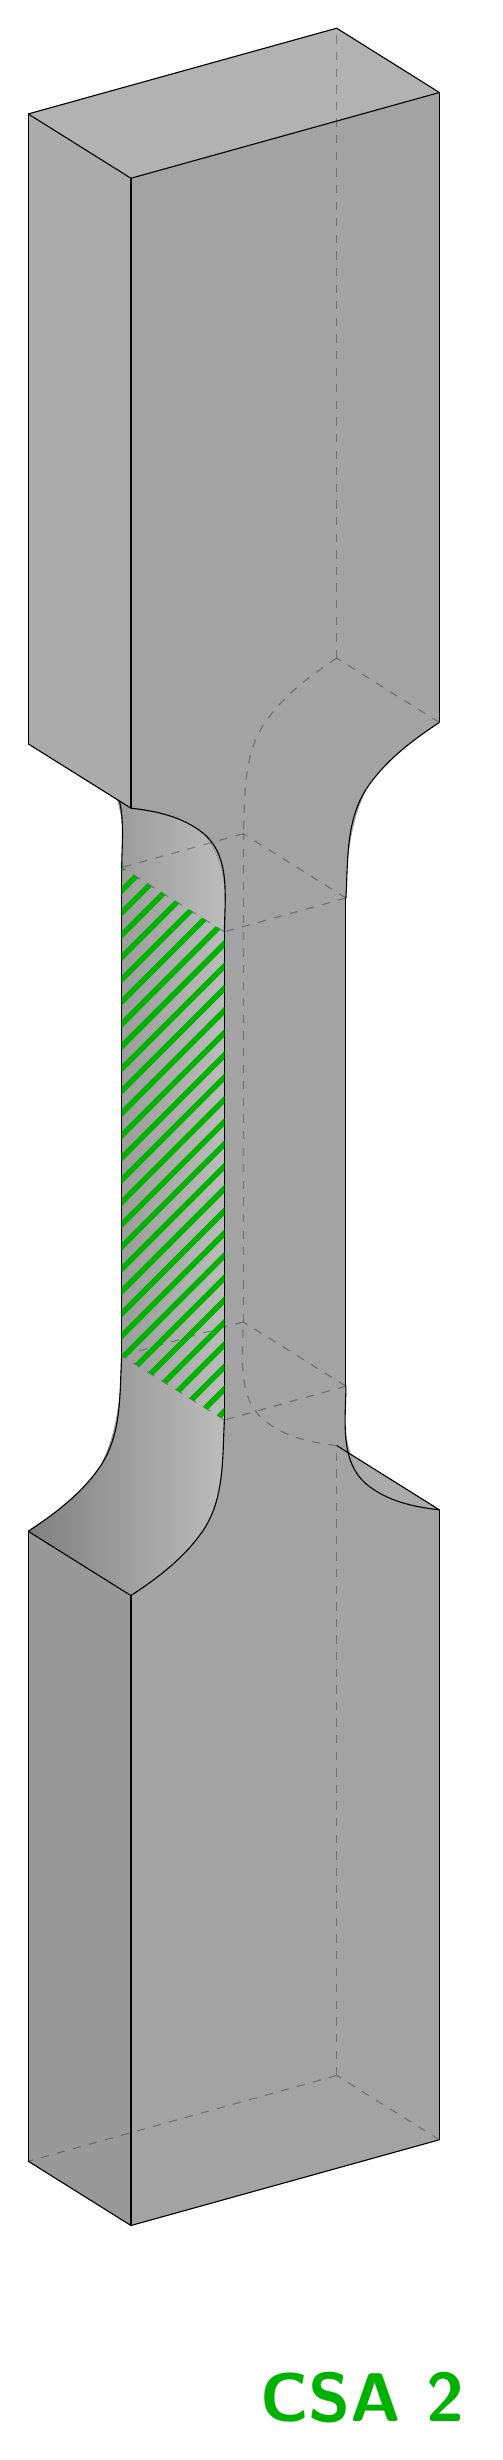
\begin{tikzpicture}[rotate around y=225, use Hobby shortcut]
    \large
    \def\width{4}
    \def\gap{10}
    \def\main{8}
    \def\curvy{1.9}
    \def\depth{3}
    
    \def\n{3.3}
    \def\z{1/\n}
    \pgfmathsetmacro{\s}{1-\z}
    
    \coordinate (A) at (0,\main,0);
    \coordinate (B) at (\width*\z-\width*\z*0.23,\main+\curvy-\curvy*0.7,0);
    \coordinate (C) at (\width*\z,\main+\curvy,0);
    
    \coordinate (A2) at (\width,\main,0);
    \coordinate (B2) at (\width*\s+\width*\z*0.23,\main+\curvy-\curvy*0.7,0);
    \coordinate (C2) at (\width*\s,\main+\curvy,0);
    
    \coordinate (A3) at (0,\main+\gap,0);
    \coordinate (B3) at (\width*\z-\width*\z*0.23,\main+\gap-\curvy+\curvy*0.7,0);
    \coordinate (C3) at (\width*\z,\main+\gap-\curvy,0);
    
    \coordinate (A4) at (\width,\main+\gap,0);
    \coordinate (B4) at (\width*\s+\width*\z*0.23,\main+\gap-\curvy+\curvy*0.7,0);
    \coordinate (C4) at (\width*\s,\main+\gap-\curvy,0);
    
    % Back variation with \depth (subtracting \depth from the z-coordinate)
    \coordinate (A') at (0,\main,\depth);
    \coordinate (B') at (\width*\z-\width*\z*0.23,\main+\curvy-\curvy*0.7,\depth);
    \coordinate (C') at (\width*\z,\main+\curvy,\depth);
    
    \coordinate (A2') at (\width,\main,\depth);
    \coordinate (B2') at (\width*\s+\width*\z*0.23,\main+\curvy-\curvy*0.7,\depth);
    \coordinate (C2') at (\width*\s,\main+\curvy,\depth);
    
    \coordinate (A3') at (0,\main+\gap,\depth);
    \coordinate (B3') at (\width*\z-\width*\z*0.23,\main+\gap-\curvy+\curvy*0.7,\depth);
    \coordinate (C3') at (\width*\z,\main+\gap-\curvy,\depth);
    
    \coordinate (A4') at (\width,\main+\gap,\depth);
    \coordinate (B4') at (\width*\s+\width*\z*0.23,\main+\gap-\curvy+\curvy*0.7,\depth);
    \coordinate (C4') at (\width*\s,\main+\gap-\curvy,\depth);
    
    
    % Back face fill
    \fill[black!40] 
    (0,0,\depth) -- (\width,0,\depth) -- (\width,\main,\depth) 
    to[hobby,tension=3] (\width,\main,\depth) .. (\width*\s+\width*\z*0.23,\main+\curvy-\curvy*0.7,\depth) .. (\width*\s,\main+\curvy,\depth) -- 
    (\width*\s,\main+\gap-\curvy,\depth) 
    to[hobby,tension=3] (\width*\s,\main+\gap-\curvy,\depth)  .. (\width*\s+\width*\z*0.23,\main+\gap-\curvy+\curvy*0.7,\depth) .. (\width,\main+\gap,\depth) --
    (\width,2*\main+\gap,\depth) -- (0,2*\main+\gap,\depth) -- 
    (0,\main+\gap,\depth) to[hobby,tension=3] (0,\main+\gap,\depth) .. (\width*\z-\width*\z*0.23,\main+\gap-\curvy+\curvy*0.7,\depth) .. (\width*\z,\main+\gap-\curvy,\depth) --
    (\width*\z,\main+\curvy,\depth) to[hobby,tension=3] (\width*\z,\main+\curvy,\depth) .. (\width*\z-\width*\z*0.23,\main+\curvy-\curvy*0.7,\depth) .. (0,\main,\depth) --
    cycle;
    
    % Curves fills with refined fades
    \fill[left color=gray!80, middle color=gray!50, right color=gray!20, opacity=0.8] 
    (A) to[hobby,tension=3] (A) .. (B) .. (C) -- (C3) to[hobby,tension=3] (C3) .. (B3) .. (A3) -- 
    (A3') to[hobby,tension=3] (A3') .. (B3') .. (C3') --
    (C') to[hobby,tension=3] (C') .. (B') .. (A') -- cycle;
    
    \fill[left color=gray!80, middle color=gray!50, right color=gray!20, opacity=0.8] 
    (A2) to[hobby,tension=3] (A2) .. (B2) .. (C2) -- (C4) to[hobby,tension=3] (C4) .. (B4) .. (A4) -- 
    (A4') to[hobby,tension=3] (A4') .. (B4') .. (C4') --
    (C2') to[hobby,tension=3] (C2') .. (B2') .. (A2') -- cycle;
    
    
    \draw[-,hobby,tension=3] (A2') .. (B2') .. (C2');
    \draw[-,hobby,tension=3] (A4') .. (B4') .. (C4');
    
    % Fill for bottom rectangle section
    \fill[black!33] 
    (0,0,0) -- (\width,0,0) -- (\width,0,\depth) -- (0,0,\depth) -- cycle;
    \fill[black!33] 
    (0,0,0) -- (0,\main,0) -- (0,\main,\depth) -- (0,0,\depth) -- cycle;
    \fill[black!40] 
    (\width,0,0) -- (\width,\main,0) -- (\width,\main,\depth) -- (\width,0,\depth) -- cycle;
    
    % Fill for top rectangle section
    \fill[black!30] 
    (0,2*\main+\gap,0) -- (\width,2*\main+\gap,0) -- (\width,2*\main+\gap,\depth) -- (0,2*\main+\gap,\depth) -- cycle;
    \fill[black!30] 
    (0,\main+\gap,0) -- (0,2*\main+\gap,0) -- (0,2*\main+\gap,\depth) -- (0,\main+\gap,\depth) -- cycle;
    \fill[black!33] 
    (\width,\main+\gap,0) -- (\width,2*\main+\gap,0) -- (\width,2*\main+\gap,\depth) -- (\width,\main+\gap,\depth) -- cycle;
    
    
    
    % Front face fill
    \fill[black!36] 
    (0,0,0) -- (\width,0,0) -- (\width,\main,0) 
    to[hobby,tension=3] (A2) .. (B2) .. (C2) -- 
    (\width*\s,\main+\gap-\curvy,0) 
    to[hobby,tension=3] (C4) .. (B4) .. (A4) --
    (\width,2*\main+\gap,0) -- (0,2*\main+\gap,0) -- 
    (0,\main+\gap,0) to[hobby,tension=3] (A3) .. (B3) .. (C3) --
    (\width*\z,\main+\curvy,0) to[hobby,tension=3] (C) .. (B) .. (A) --
    cycle;
    \draw[hobby,tension=3] (A) .. (B) .. (C);
    \draw[hobby,tension=3] (A2) .. (B2) .. (C2);
    \draw[hobby,tension=3] (A3) .. (B3) .. (C3);
    \draw[hobby,tension=3] (A4) .. (B4) .. (C4);
    \draw[dashed, opacity=0.3,hobby,tension=3] (A3') .. (B3') .. (C3');
    \draw[dashed, opacity=0.3,hobby,tension=3] (A') .. (B') .. (C');
    % Front face outline
    
    \draw[-] (0,0,0) -- (\width,0,0);
    \draw[-] (0,0,0) -- (0,\main,0);
    \draw[-] (\width*\z,\main+\curvy,0) -- (\width*\z,\main+\gap-\curvy,0);
    \draw[-] (0,\main+\gap,0) -- (0,2*\main+\gap,0);
    \draw[-] (0,2*\main+\gap,0) -- (\width,2*\main+\gap,0);
    \draw[-] (\width,2*\main+\gap,0) -- (\width,\main+\gap,0);
    \draw[-] (\width*\s,\main+\curvy,0) -- (\width*\s,\main+\gap-\curvy,0);    
    \draw[-] (\width,0,0) -- (\width,\main,0);
    
    
    
    
    
    % Back face outline
    
    
    \draw[dashed, opacity=0.3] (\width*\z,\main+\curvy,\depth) -- (\width*\z,\main+\gap-\curvy,\depth);
    \draw[-] (\width*\s,\main+\curvy,\depth) -- (\width*\s,\main+\gap-\curvy,\depth);
    \draw[dashed, opacity=0.3] (0,0,\depth) -- (\width,0,\depth);
    \draw[dashed, opacity=0.3] (0,0,\depth) -- (0,\main,\depth);
    \draw[-] (\width,0,\depth) -- (\width,\main,\depth);
    \draw[dashed, opacity=0.3] (0,\main+\gap,\depth) -- (0,2*\main+\gap,\depth);
    \draw[-] (0,2*\main+\gap,\depth) -- (\width,2*\main+\gap,\depth);
    \draw[-] (\width,2*\main+\gap,\depth) -- (\width,\main+\gap,\depth);
    
    
    
    % Connect front and back faces
    %botom
    \draw[-] (\width,\main,0) -- (\width,\main,\depth);
    \draw[-] (\width,0,0) -- (\width,0,\depth);
    \draw[dashed, opacity=0.3] (0,0,0) -- (0,0,\depth);
    \draw[-] (0,\main,0) -- (0,\main,\depth);
    %top
    \draw[-] (\width,\main+\gap,0) -- (\width,\main+\gap,\depth);
    \draw[-] (\width,2*\main+\gap,0) -- (\width,2*\main+\gap,\depth);
    \draw[-] (0,2*\main+\gap,0) -- (0,2*\main+\gap,\depth);
    \draw[dashed, opacity=0.3] (0,\main+\gap,0) -- (0,\main+\gap,\depth);
    
    
    
    %curves
    \draw[dashed, opacity=0.3] (C) -- (C2);
    \draw[dashed, opacity=0.3] (C3) -- (C4);
    \draw[dashed, opacity=0.3] (C') -- (C2');
    \draw[dashed, opacity=0.3] (C3') -- (C4');
    \draw[dashed, opacity=0.3] (C) -- (C');
    \draw[dashed, opacity=0.3] (C2) -- (C2');
    \draw[dashed, opacity=0.3] (C3) -- (C3');
    \draw[dashed, opacity=0.3] (C4) -- (C4');
    
    
    \fill[pattern={Lines[
        distance=2mm,
        angle=45,
        line width=0.7mm
        ]},
    pattern color=green!70!black
    ] (C2) -- (C4) -- (C4') -- (C2') -- cycle;
    \node at (1,-3,0) {\Huge \color{green!70!black}\textbf{\textsf{CSA 2}}};
\end{tikzpicture}
\vspace{5em}
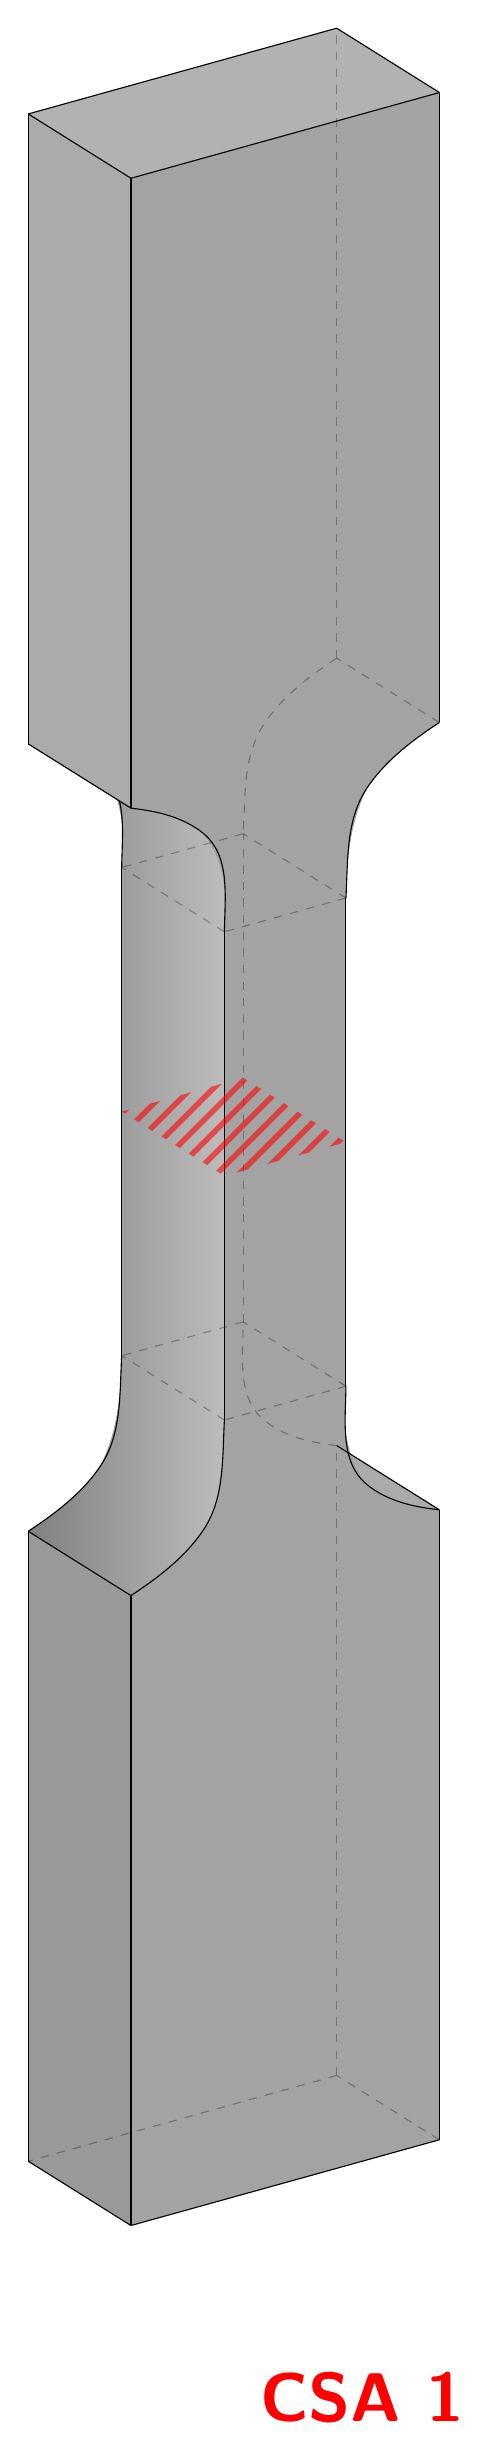
\begin{tikzpicture}[rotate around y=225, use Hobby shortcut]
    \large
    \def\width{4}
    \def\gap{10}
    \def\main{8}
    \def\curvy{1.9}
    \def\depth{3}
    
    \def\n{3.3}
    \def\z{1/\n}
    \pgfmathsetmacro{\s}{1-\z}
    
    \coordinate (A) at (0,\main,0);
    \coordinate (B) at (\width*\z-\width*\z*0.23,\main+\curvy-\curvy*0.7,0);
    \coordinate (C) at (\width*\z,\main+\curvy,0);
    
    \coordinate (A2) at (\width,\main,0);
    \coordinate (B2) at (\width*\s+\width*\z*0.23,\main+\curvy-\curvy*0.7,0);
    \coordinate (C2) at (\width*\s,\main+\curvy,0);
    
    \coordinate (A3) at (0,\main+\gap,0);
    \coordinate (B3) at (\width*\z-\width*\z*0.23,\main+\gap-\curvy+\curvy*0.7,0);
    \coordinate (C3) at (\width*\z,\main+\gap-\curvy,0);

    \coordinate (A4) at (\width,\main+\gap,0);
    \coordinate (B4) at (\width*\s+\width*\z*0.23,\main+\gap-\curvy+\curvy*0.7,0);
    \coordinate (C4) at (\width*\s,\main+\gap-\curvy,0);
    
    % Back variation with \depth (subtracting \depth from the z-coordinate)
    \coordinate (A') at (0,\main,\depth);
    \coordinate (B') at (\width*\z-\width*\z*0.23,\main+\curvy-\curvy*0.7,\depth);
    \coordinate (C') at (\width*\z,\main+\curvy,\depth);
    
    \coordinate (A2') at (\width,\main,\depth);
    \coordinate (B2') at (\width*\s+\width*\z*0.23,\main+\curvy-\curvy*0.7,\depth);
    \coordinate (C2') at (\width*\s,\main+\curvy,\depth);
    
    \coordinate (A3') at (0,\main+\gap,\depth);
    \coordinate (B3') at (\width*\z-\width*\z*0.23,\main+\gap-\curvy+\curvy*0.7,\depth);
    \coordinate (C3') at (\width*\z,\main+\gap-\curvy,\depth);
    
    \coordinate (A4') at (\width,\main+\gap,\depth);
    \coordinate (B4') at (\width*\s+\width*\z*0.23,\main+\gap-\curvy+\curvy*0.7,\depth);
    \coordinate (C4') at (\width*\s,\main+\gap-\curvy,\depth);
    
    
    % Back face fill
    \fill[black!40] 
    (0,0,\depth) -- (\width,0,\depth) -- (\width,\main,\depth) 
    to[hobby,tension=3] (\width,\main,\depth) .. (\width*\s+\width*\z*0.23,\main+\curvy-\curvy*0.7,\depth) .. (\width*\s,\main+\curvy,\depth) -- 
    (\width*\s,\main+\gap-\curvy,\depth) 
    to[hobby,tension=3] (\width*\s,\main+\gap-\curvy,\depth)  .. (\width*\s+\width*\z*0.23,\main+\gap-\curvy+\curvy*0.7,\depth) .. (\width,\main+\gap,\depth) --
    (\width,2*\main+\gap,\depth) -- (0,2*\main+\gap,\depth) -- 
    (0,\main+\gap,\depth) to[hobby,tension=3] (0,\main+\gap,\depth) .. (\width*\z-\width*\z*0.23,\main+\gap-\curvy+\curvy*0.7,\depth) .. (\width*\z,\main+\gap-\curvy,\depth) --
    (\width*\z,\main+\curvy,\depth) to[hobby,tension=3] (\width*\z,\main+\curvy,\depth) .. (\width*\z-\width*\z*0.23,\main+\curvy-\curvy*0.7,\depth) .. (0,\main,\depth) --
    cycle;
    
    % Curves fills with refined fades
    \fill[left color=gray!80, middle color=gray!50, right color=gray!20, opacity=0.8] 
    (A) to[hobby,tension=3] (A) .. (B) .. (C) -- (C3) to[hobby,tension=3] (C3) .. (B3) .. (A3) -- 
    (A3') to[hobby,tension=3] (A3') .. (B3') .. (C3') --
    (C') to[hobby,tension=3] (C') .. (B') .. (A') -- cycle;
    
    \fill[left color=gray!80, middle color=gray!50, right color=gray!20, opacity=0.8] 
    (A2) to[hobby,tension=3] (A2) .. (B2) .. (C2) -- (C4) to[hobby,tension=3] (C4) .. (B4) .. (A4) -- 
    (A4') to[hobby,tension=3] (A4') .. (B4') .. (C4') --
    (C2') to[hobby,tension=3] (C2') .. (B2') .. (A2') -- cycle;
    
    
    \draw[-,hobby,tension=3] (A2') .. (B2') .. (C2');
    \draw[-,hobby,tension=3] (A4') .. (B4') .. (C4');
    
    % Fill for bottom rectangle section
    \fill[black!33] 
    (0,0,0) -- (\width,0,0) -- (\width,0,\depth) -- (0,0,\depth) -- cycle;
    \fill[black!33] 
    (0,0,0) -- (0,\main,0) -- (0,\main,\depth) -- (0,0,\depth) -- cycle;
    \fill[black!40] 
    (\width,0,0) -- (\width,\main,0) -- (\width,\main,\depth) -- (\width,0,\depth) -- cycle;
    
    % Fill for top rectangle section
    \fill[black!30] 
    (0,2*\main+\gap,0) -- (\width,2*\main+\gap,0) -- (\width,2*\main+\gap,\depth) -- (0,2*\main+\gap,\depth) -- cycle;
    \fill[black!30] 
    (0,\main+\gap,0) -- (0,2*\main+\gap,0) -- (0,2*\main+\gap,\depth) -- (0,\main+\gap,\depth) -- cycle;
    \fill[black!33] 
    (\width,\main+\gap,0) -- (\width,2*\main+\gap,0) -- (\width,2*\main+\gap,\depth) -- (\width,\main+\gap,\depth) -- cycle;
    
    
    
    % Front face fill
    \fill[black!36] 
    (0,0,0) -- (\width,0,0) -- (\width,\main,0) 
    to[hobby,tension=3] (A2) .. (B2) .. (C2) -- 
    (\width*\s,\main+\gap-\curvy,0) 
    to[hobby,tension=3] (C4) .. (B4) .. (A4) --
    (\width,2*\main+\gap,0) -- (0,2*\main+\gap,0) -- 
    (0,\main+\gap,0) to[hobby,tension=3] (A3) .. (B3) .. (C3) --
    (\width*\z,\main+\curvy,0) to[hobby,tension=3] (C) .. (B) .. (A) --
    cycle;
    \draw[hobby,tension=3] (A) .. (B) .. (C);
    \draw[hobby,tension=3] (A2) .. (B2) .. (C2);
    \draw[hobby,tension=3] (A3) .. (B3) .. (C3);
    \draw[hobby,tension=3] (A4) .. (B4) .. (C4);
    \draw[dashed, opacity=0.3,hobby,tension=3] (A3') .. (B3') .. (C3');
    \draw[dashed, opacity=0.3,hobby,tension=3] (A') .. (B') .. (C');
    % Front face outline
    
    \draw[-] (0,0,0) -- (\width,0,0);
    \draw[-] (0,0,0) -- (0,\main,0);
    \draw[-] (\width*\z,\main+\curvy,0) -- (\width*\z,\main+\gap-\curvy,0);
    \draw[-] (0,\main+\gap,0) -- (0,2*\main+\gap,0);
    \draw[-] (0,2*\main+\gap,0) -- (\width,2*\main+\gap,0);
    \draw[-] (\width,2*\main+\gap,0) -- (\width,\main+\gap,0);
    \draw[-] (\width*\s,\main+\curvy,0) -- (\width*\s,\main+\gap-\curvy,0);    
    \draw[-] (\width,0,0) -- (\width,\main,0);
    
    
    
    
    
    % Back face outline
    
    
    \draw[dashed, opacity=0.3] (\width*\z,\main+\curvy,\depth) -- (\width*\z,\main+\gap-\curvy,\depth);
    \draw[-] (\width*\s,\main+\curvy,\depth) -- (\width*\s,\main+\gap-\curvy,\depth);
    \draw[dashed, opacity=0.3] (0,0,\depth) -- (\width,0,\depth);
    \draw[dashed, opacity=0.3] (0,0,\depth) -- (0,\main,\depth);
    \draw[-] (\width,0,\depth) -- (\width,\main,\depth);
    \draw[dashed, opacity=0.3] (0,\main+\gap,\depth) -- (0,2*\main+\gap,\depth);
    \draw[-] (0,2*\main+\gap,\depth) -- (\width,2*\main+\gap,\depth);
    \draw[-] (\width,2*\main+\gap,\depth) -- (\width,\main+\gap,\depth);
    
    
    
    % Connect front and back faces
    %botom
    \draw[-] (\width,\main,0) -- (\width,\main,\depth);
    \draw[-] (\width,0,0) -- (\width,0,\depth);
    \draw[dashed, opacity=0.3] (0,0,0) -- (0,0,\depth);
    \draw[-] (0,\main,0) -- (0,\main,\depth);
    %top
    \draw[-] (\width,\main+\gap,0) -- (\width,\main+\gap,\depth);
    \draw[-] (\width,2*\main+\gap,0) -- (\width,2*\main+\gap,\depth);
    \draw[-] (0,2*\main+\gap,0) -- (0,2*\main+\gap,\depth);
    \draw[dashed, opacity=0.3] (0,\main+\gap,0) -- (0,\main+\gap,\depth);
    
    
    
    %curves
    \draw[dashed, opacity=0.3] (C) -- (C2);
    \draw[dashed, opacity=0.3] (C3) -- (C4);
    \draw[dashed, opacity=0.3] (C') -- (C2');
    \draw[dashed, opacity=0.3] (C3') -- (C4');
    \draw[dashed, opacity=0.3] (C) -- (C');
    \draw[dashed, opacity=0.3] (C2) -- (C2');
    \draw[dashed, opacity=0.3] (C3) -- (C3');
    \draw[dashed, opacity=0.3] (C4) -- (C4');
    
   \pgfmathsetmacro{\halfgap}{0.5*\gap}

   \coordinate (C3m) at (\width*\z,\main+\halfgap,0);
   \coordinate (C4m) at (\width*\s,\main+\halfgap,0);
   \coordinate (C3'm) at (\width*\z,\main+\halfgap,\depth);
   \coordinate (C4'm) at (\width*\s,\main+\halfgap,\depth);
    
    \fill[pattern={Lines[
        distance=2mm,
        angle=45,
        line width=0.7mm
        ]},
    pattern color=red,
    opacity=0.6] (C3m) -- (C3'm) -- (C4'm) -- (C4m) -- cycle;
    \node at (1,-3,0) {\Huge \color{red}\textbf{\textsf{CSA 1}}};
\end{tikzpicture}

\end{document}